\documentclass[12pt,
%answers
]{exam}
\usepackage[margin=.8 in]{geometry} 
\usepackage{hyperref,enumerate}
\usepackage{tikz}
\usepackage{amsmath,graphicx, color,comment,amssymb,multicol,cancel}
\newcommand{\tit}{\textit}
\newcommand{\tbf}{\textbf}
\newcommand{\notimplies}{%
  \mathrel{{\ooalign{\hidewidth$\not\phantom{=}$\hidewidth\cr$\implies$}}}}
\newcommand{\ds}{\displaystyle}
\newcommand{\dstyle}{\ds}
\newcommand{\lt}{\left}
\newcommand{\rt}{\right}
\newcommand{\qtq}[1] {\quad \text{#1}\quad}
\newcommand{\Lt}[1]{\mathcal{L} \lt\{ {#1} \rt\}}
\newcommand{\Lti}[1]{\mathcal{L}^{-1} \lt\{ {#1} \rt\}}
\renewcommand{\v}[1]{\vec{\mathbf{#1}}}
\newcommand{\mb}{\mathbf}
\newcommand{\inverse}[1]{ {\mb{#1}}^{-1} }
\makeatletter
\renewcommand*\env@matrix[1][*\c@MaxMatrixCols c]{%
  \hskip -\arraycolsep
  \let\@ifnextchar\new@ifnextchar
  \array{#1}}
\makeatother
\renewcommand{\v}[1]{\vec{\mathbf{#1}}}
\newcommand{\derv}[1]{\vec{\mathbf{#1}}\,' }


\newcounter{quest}


  
% ---- Change the information below ----------------------------------------------------------------------------
\newcommand{\worksheetdate}{ 2024}
%\newcommand{\worksheetdue}{Wednesday, August 24, 2016}
\newcommand{\coursetitle}{}
\newcommand{\worksheettitle}{Graphs of exponential functions}
\newcommand{\worksheetsection}{}
% ---- Change the information above ----------------------------------------------------------------------------


%%% adjust space above and below displaymath
\abovedisplayshortskip=0.5em
\belowdisplayshortskip=0.75em
\abovedisplayskip=0.5em
\belowdisplayskip=0.75em
%%% adjust space above and below displaymath


\pagestyle{head}
\runningheadrule \firstpageheader
{\fbox{\parbox{.5\textwidth}{
\textbf{\small Your Name: }
\\ \\ \\ 
%\textbf{Your Name:}
\\
}}}
{}
{\parbox{1.1in}{\fbox{ \parbox{1in}{ \textbf{\small ID \#:  \\  \\ \\ } }}
%\fbox{ \parbox{1in}{ \textbf{\small Section:  \\  } }}
 }}
\runningheader
{{}}%
{\worksheetsection  Page \thepage\ of \numpages}
{\textbf{} \hphantom{\worksheetdate}}

\begin{document}

\newgeometry{top=1.3in, right =0.8in, left=0.8in, bottom =0.8in}

\begin{center}	
{\bf {\coursetitle\,  Worksheet: \worksheettitle} 
	\\ 
	\textbf{}
	\hphantom{\worksheetdate}
%	\worksheetdate
} 		
	\end{center}




\begin{questions}

%%% adjust space above and below displaymath
\abovedisplayshortskip=0.5em
\belowdisplayshortskip=0.75em
\abovedisplayskip=0.5em
\belowdisplayskip=0.75em
%%% adjust space above and below displaymath

\question
 Select the graph for the  function $f(x)=(\frac{1}{8})^x$
 
         \includegraphics[width=3.5cm]{Images/gepic1.png}
     \includegraphics[width=3.5cm]{Images/gepic2.png}
          \includegraphics[width=3.5cm]{Images/gepic3.png}
               \includegraphics[width=3.5cm]{Images/gepic4.png}
                    \includegraphics[width=3.5cm]{Images/gepic5.png}
   
  ~\hspace{1cm} (A) \hspace{2.5cm} (B)  \hspace{2.8cm} (C) \hspace{3cm} (D) \hspace{3cm} (E)
 
 \question
  Identify the graphs of the functions $y=2^x$ and  $y=4^x$
  
    \includegraphics[width=3.5cm]{Images/gepic6.png}
     \includegraphics[width=3.5cm]{Images/gepic7.png}
          \includegraphics[width=3.5cm]{Images/gepic8.png}
               \includegraphics[width=3.5cm]{Images/gepic9.png}
                    \includegraphics[width=3.5cm]{Images/gepic10.png}
   
  ~\hspace{1cm} (A) \hspace{2.5cm} (B)  \hspace{2.8cm} (C) \hspace{3cm} (D) \hspace{3cm} (E)


\question
Find the exponential function $f(x)=a^x$ whose graph is given.
\begin{multicols}{2}
\begin{center}
       \includegraphics[width=3.5cm]{Images/gepic11.png}
 \end{center}
\columnbreak
\begin{choices}
\choice $f(x)=3^x$
\choice $f(x)=3^{x+3}$
\choice $f(x)=-3^{x}$
\choice $f(x)=3^{-x}$
\choice $f(x)=x^3$
\end{choices}

\end{multicols}


\question
Determine the graph of the function $y=4^{x+2}$

\includegraphics[width=3.5cm]{Images/gepic12.png}
     \includegraphics[width=3.5cm]{Images/gepic13.png}
          \includegraphics[width=3.5cm]{Images/gepic14.png}
               \includegraphics[width=3.5cm]{Images/gepic15.png}
                    \includegraphics[width=3.5cm]{Images/gepic16.png}
   
  ~\hspace{1cm} (A) \hspace{2.5cm} (B)  \hspace{2.8cm} (C) \hspace{3cm} (D) \hspace{3cm} (E)


\question
Determine the graph of the function $f(x)=11^{x+3}$

\begin{tabular}{ccccc}
\includegraphics[width=3cm]{Images/gepic17.png}&
     \includegraphics[width=3cm]{Images/gepic18.png}&
          \includegraphics[width=3cm]{Images/gepic19.png}&
               \includegraphics[width=3cm]{Images/gepic20.png}&
                    \includegraphics[width=3cm]{Images/gepic21.png}\\
  \footnotesize  Domain: $(-\infty, \infty)$ &     Domain: $(-\infty, \infty)$ &     Domain: $(-\infty, \infty)$&   Domain: $(0, \infty)$&    Domain: $(0, \infty)$\\
    Range: $(0, \infty)$  & Range: $(0, \infty)$ &Range: $(0, \infty)$  & Range: $(-\infty, \infty)$ & Range: $(-\infty, \infty)$ \\
    Asymptote: $y = 0$&
Asymptote: $x = 0$&
Asymptote: $y = 0$&
Asymptote: $y = 0$&
Asymptote: $y = 0$\\
    \end{tabular}
   
  ~\hspace{1cm} (A) \hspace{2.5cm} (B)  \hspace{2.8cm} (C) \hspace{3cm} (D) \hspace{3cm} (E)



\question
Determine the graph of the function $f(x)=-(\frac{1}{10})^x$

\begin{tabular}{ccccc}
\includegraphics[width=3cm]{Images/gepic22.png}&
     \includegraphics[width=3cm]{Images/gepic23.png}&
          \includegraphics[width=3cm]{Images/gepic24.png}&
               \includegraphics[width=3cm]{Images/gepic25.png}&
                    \includegraphics[width=3cm]{Images/gepic26.png}\\
  \footnotesize  Domain: $(-\infty, \infty)$ &     Domain: $(-\infty, 0)$ &     Domain: $(-\infty, 0)$&   Domain: $(-\infty, 0)$&    Domain: $(-\infty,  \infty)$ \\
    Range: $(-\infty, 0)$  & Range: $(-\infty, \infty)$ &Range: $(-\infty, \infty)$  & Range: $(-\infty, \infty)$ & Range: $(-\infty, 0)$ \\
    Asymptote: $x = 0$& Asymptote: $x = 0$& Asymptote: $x = 0$& Asymptote: $y = 0$& Asymptote: $y = 0$\\
    \end{tabular}
   
  ~\hspace{1cm} (A) \hspace{2.5cm} (B)  \hspace{2.8cm} (C) \hspace{3cm} (D) \hspace{3cm} (E)



\question
Based on the given graph of $f(x)=3^x$, graph $g(x)=3^{-x}$ and $h(x)=3^{x-1}+1$

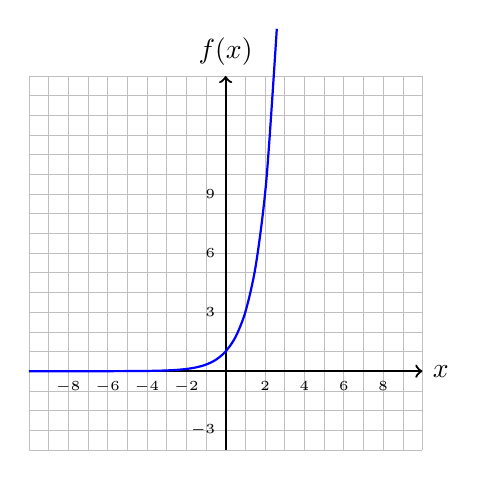
\begin{tikzpicture}[scale=0.25]
\draw[help lines, color=gray!50] (-10,-4) grid (10,15);
\draw[->,thick] (-10,0)--(10,0) node[right]{$x$};
\draw[->, thick] (0,-4)--(0,15) node[above]{$f(x)$};
\foreach \x in {-8,-6,-4,-2,2,4,6,8}
\draw (\x cm,0.25pt) -- (\x cm,-0.25 pt) node[anchor=north] {\tiny{$\x$}};
\foreach \y in {-3,3,6,9}
\draw (1pt,\y cm) -- (-1pt,\y cm) node[anchor=east] {\tiny{$\y$}};
\draw[scale=1, domain=-10:2.6, smooth, variable=\x, thick, blue] plot ({\x},{3^ (\x)});
\end{tikzpicture}


\end{questions}
\end{document}






